% Figure: diffusion / score / flow matching in one frame.
% Teaching point: training regresses ONE local target at ONE random time slice,
% while sampling is a LONG integration -- run in reverse time for diffusion
% (noise -> data) but forward in time for flow matching (base -> data).
% Design width ~168mm.
\documentclass[border=0pt]{standalone}
\usepackage{amsmath,amssymb}
% Shared visual language for the figures of the book.
% Every figure in this directory loads this file so the chapter reads as one system.
% NOTE: no blank lines are allowed inside \tikzset{...} (a blank line emits \par
% and breaks key scanning).
\NeedsTeXFormat{LaTeX2e}
\ProvidesPackage{figstyle}[2026/10/21 Figure style for Free Energy to LLMs]

\RequirePackage{tikz}
\usetikzlibrary{arrows.meta,positioning,calc,fit,shapes.geometric,shapes.misc,%
  backgrounds,matrix,decorations.pathreplacing,decorations.markings,patterns.meta}

% ---------------------------------------------------------------- palette
% Same values as book/preamble/style.tex, prefixed with F.
\definecolor{FNavy}{HTML}{14324A}
\definecolor{FTeal}{HTML}{0E7490}
\definecolor{FSky}{HTML}{E7F5F8}
\definecolor{FOrange}{HTML}{D97706}
\definecolor{FAmber}{HTML}{FFF3D6}
\definecolor{FInk}{HTML}{1F2937}
\definecolor{FSlate}{HTML}{64748B}
\definecolor{FMist}{HTML}{F5F7FA}
\definecolor{FRose}{HTML}{9F1239}
\definecolor{FRoseMist}{HTML}{FFF1F2}

% ---------------------------------------------------------------- semantics
% Teal   = probability / model / data object
% Orange = training objective, cost, or the quantity moved through the system
% Navy   = neutral structure
% Slate  = secondary label or metadata
% Rose   = failure mode, hazard, masked-out region
\tikzset{
  % Lay figures out in millimetres.  A figure designed 168mm wide is included at
  % \textwidth, so its fonts appear at exactly the size written here.
  every picture/.style={x=1mm,y=1mm,font=\small,line cap=round,line join=round},
  % ---- block styles
  nbase/.style={draw,rounded corners=1.2pt,align=center,inner sep=2.4pt,%
    minimum height=7mm,text=FInk},
  nteal/.style={nbase,draw=FTeal,fill=FSky},
  norange/.style={nbase,draw=FOrange,fill=FAmber},
  nnavy/.style={nbase,draw=FNavy,fill=white},
  nsoft/.style={nbase,draw=FSlate!55,fill=FMist},
  nrose/.style={nbase,draw=FRose,fill=FRoseMist},
  ghost/.style={draw=none,fill=none,align=center,inner sep=1pt},
  plain/.style={draw=none,fill=none,align=center,inner sep=0pt},
  % ---- arrows
  ar/.style={-{Latex[length=1.7mm,width=1.35mm]},draw=FSlate,line width=0.75pt},
  ard/.style={ar,dashed},
  arteal/.style={ar,draw=FTeal},
  arorange/.style={ar,draw=FOrange},
  arrose/.style={ar,draw=FRose},
  thickar/.style={ar,line width=1.2pt},
  % ---- text roles
  ftitle/.style={font=\large\bfseries,text=FNavy,align=center},
  ptitle/.style={font=\small\bfseries,text=FNavy,align=center},
  ptitleo/.style={font=\small\bfseries,text=FOrange,align=center},
  lbl/.style={font=\scriptsize,text=FSlate,align=center,inner sep=1pt},
  lblt/.style={lbl,text=FTeal},
  lblo/.style={lbl,text=FOrange},
  lbln/.style={lbl,text=FNavy},
  lblr/.style={lbl,text=FRose},
  sub/.style={font=\scriptsize,text=FSlate!90,align=center,inner sep=1pt},
  monob/.style={font=\ttfamily\scriptsize,text=FInk,inner sep=1pt},
  mathb/.style={font=\small,text=FInk,inner sep=1pt},
  eqn/.style={font=\scriptsize,inner sep=1.5pt,text=FInk},
  % ---- decorations
  brace/.style={decorate,decoration={brace,amplitude=2.4pt},draw=FSlate,%
    line width=0.6pt},
  bracet/.style={brace,draw=FTeal},
  braceo/.style={brace,draw=FOrange},
  axis/.style={draw=FSlate!55,line width=0.6pt},
  guide/.style={draw=FSlate!45,line width=0.5pt,dashed},
  halolabel/.style={font=\scriptsize,text=FInk,fill=white,fill opacity=0.85,%
    text opacity=1,inner sep=1.4pt,align=center},
}

% Figure title above the drawing, anchored at the figure's top-left.
\newcommand{\figtitle}[2][0]{%
  \node[ftitle,anchor=north west,outer sep=0pt] at (#1,0) {#2};}

% Rounded panel behind a subgroup of nodes.
\newcommand{\figpanel}[3][]{%
  \node[draw=FSlate!35,fill=#3,rounded corners=2pt,inner sep=2.6mm,#1] {#2};}

\endinput

\begin{document}
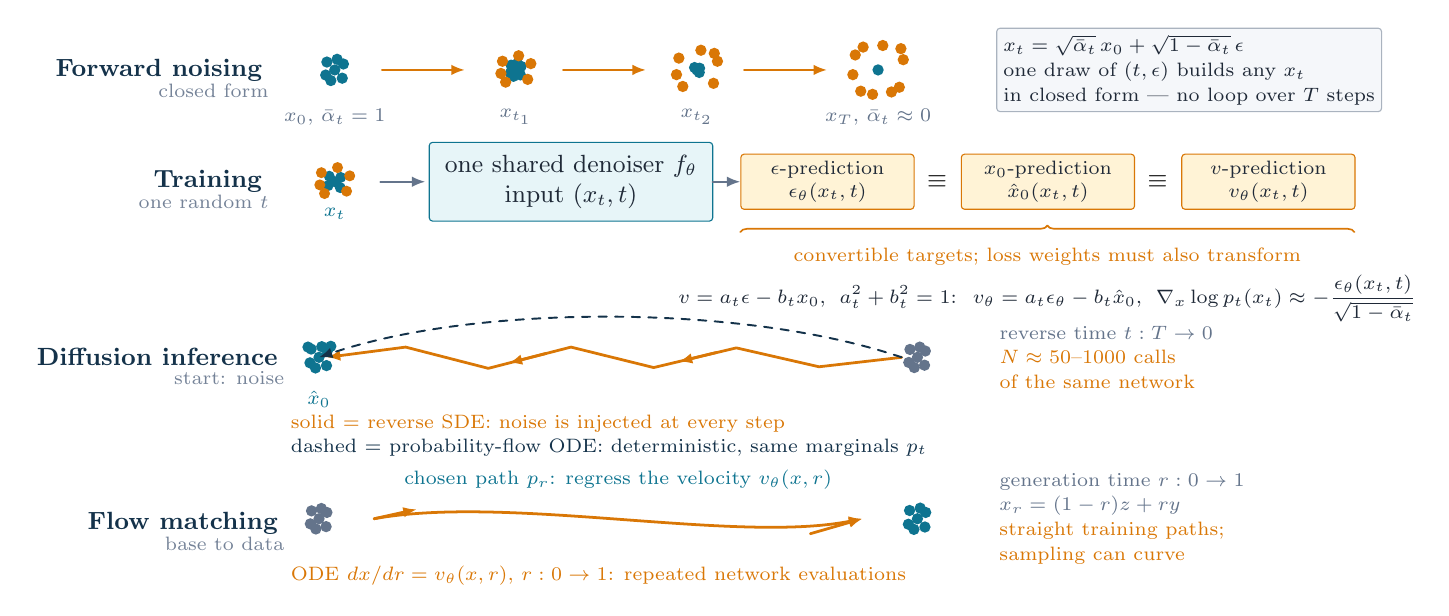
\begin{tikzpicture}
% ========================= ROW 1: forward noising -- closed form, no loop
\node[ptitle,anchor=east] at (28,53) {Forward noising};
\node[sub,anchor=east] at (28,50.4) {closed form};

\foreach \dx/\dy in {0/0,1.1/0.75,-1.0/1.0,0.95/-1.05,-1.15/-0.65,0.3/1.35,-0.5/-1.35}
  {\fill[FTeal] (36+\dx,53+\dy) circle (0.72);}
\foreach \dx/\dy in {0/0,0.66/0.45,-0.6/0.6,0.57/-0.63,-0.69/-0.39,0.2/0.81,-0.3/-0.81}
  {\fill[FTeal] (59+\dx,53+\dy) circle (0.72);}
\foreach \dx/\dy in {0/0,0.33/0.22,-0.3/0.3,0.29/-0.32}
  {\fill[FTeal] (82+\dx,53+\dy) circle (0.72);}
\fill[FTeal] (105,53) circle (0.72);

\foreach \dx/\dy in {1.9/0.8,-1.7/1.1,1.5/-1.2,-1.3/-1.55,0.35/1.8,-1.9/-0.45}
  {\fill[FOrange] (59+\dx,53+\dy) circle (0.72);}
\foreach \dx/\dy in {2.6/1.1,-2.3/1.5,2.1/-1.7,-1.8/-2.1,0.5/2.5,-2.6/-0.6,2.2/2.1}
  {\fill[FOrange] (82+\dx,53+\dy) circle (0.72);}
\foreach \dx/\dy in {3.2/1.3,-2.9/1.9,2.7/-2.2,-2.2/-2.7,0.6/3.1,-3.2/-0.6,2.9/2.7,%
  -0.7/-3.1,1.7/-2.8,-1.9/2.9}
  {\fill[FOrange] (105+\dx,53+\dy) circle (0.72);}

\draw[arorange] (42,53)--(52.5,53);
\draw[arorange] (65,53)--(75.5,53);
\draw[arorange] (88,53)--(98.5,53);

\node[lbl,anchor=north] at (36,48.4) {$x_0$, $\bar\alpha_t=1$};
\node[lbl,anchor=north] at (59,48.4) {$x_{t_1}$};
\node[lbl,anchor=north] at (82,48.4) {$x_{t_2}$};
\node[lbl,anchor=north] at (105,48.4) {$x_T$, $\bar\alpha_t\approx0$};

\node[nsoft,anchor=west,align=left,font=\scriptsize] at (120,53)
  {$x_t=\sqrt{\bar\alpha_t}\,x_0+\sqrt{1-\bar\alpha_t}\,\epsilon$\\[1pt]
   one draw of $(t,\epsilon)$ builds any $x_t$\\[1pt]
   in closed form --- no loop over $T$ steps};

% ================= ROW 2: training -- one slice, one local regression target
\node[ptitle,anchor=east] at (28,38.8) {Training};
\node[sub,anchor=east] at (28,36.2) {one random $t$};

\foreach \dx/\dy in {0/0,0.75/0.55,-0.7/0.7,0.7/-0.75,-0.85/-0.5}
  {\fill[FTeal] (36+\dx,38.8+\dy) circle (0.7);}
\foreach \dx/\dy in {1.9/0.75,-1.7/1.15,1.5/-1.2,-1.3/-1.5,0.35/1.8,-1.9/-0.4}
  {\fill[FOrange] (36+\dx,38.8+\dy) circle (0.7);}
\node[lblt,anchor=north] at (36,35.9) {$x_t$};

\draw[ar] (41.8,38.8)--(47.5,38.8);
\node[nteal,minimum width=36mm,minimum height=10mm] (net) at (66,38.8)
  {one shared denoiser $f_\theta$\\input $(x_t,t)$};

\draw[ar] (84,38.8)--(87.5,38.8);
\node[norange,minimum width=22mm,anchor=west,align=center,font=\scriptsize] at (87.5,38.8)
  {$\epsilon$-prediction\\$\epsilon_\theta(x_t,t)$};
\node[plain] at (112.5,38.8) {$\equiv$};
\node[norange,minimum width=22mm,anchor=west,align=center,font=\scriptsize] at (115.5,38.8)
  {$x_0$-prediction\\$\hat x_0(x_t,t)$};
\node[plain] at (140.5,38.8) {$\equiv$};
\node[norange,minimum width=22mm,anchor=west,align=center,font=\scriptsize] at (143.5,38.8)
  {$v$-prediction\\$v_\theta(x_t,t)$};

\draw[braceo] (87.5,32.4)--(165.5,32.4);
\node[lblo,anchor=north] at (126.5,30.8)
  {convertible targets; loss weights must also transform};
\node[eqn,anchor=north] at (126.5,27.6)
  {$v=a_t\epsilon-b_t x_0$,\; $a_t^2+b_t^2=1$:\;
   $v_\theta=a_t\epsilon_\theta-b_t\hat x_0$,\;
   $\nabla_x\log p_t(x_t)\approx-\dfrac{\epsilon_\theta(x_t,t)}{\sqrt{1-\bar\alpha_t}}$};

% ============ ROW 3: diffusion inference -- reverse time, many evaluations
\node[ptitle,anchor=east] at (30,16.5) {Diffusion inference};
\node[sub,anchor=east] at (30,13.9) {start: noise};

\foreach \dx/\dy in {0/0,1.0/0.8,-0.95/1.0,0.9/-1.0,-1.1/-0.65,0.3/1.3,-0.4/-1.3}
  {\fill[FSlate] (110+\dx,16.5+\dy) circle (0.72);}
\foreach \dx/\dy in {0/0,1.05/0.8,-1.0/1.05,0.95/-1.05,-1.15/-0.7,0.35/1.35,-0.45/-1.35,1.5/1.4,-1.4/1.3}
  {\fill[FTeal] (34+\dx,16.5+\dy) circle (0.72);}
\node[lblt,anchor=north] at (34,12.6) {$\hat x_0$};

\draw[arorange,line width=1pt]
  (108,16.5)--(97.5,15.3)--(87,17.7)--(76.5,15.2)--(66,17.8)--(55.5,15.1)--(45,17.8)--(35,16.5);
\draw[arorange,line width=1pt] (84.4,17.1)--(79.7,15.95);
\draw[arorange,line width=1pt] (62.85,17.0)--(58.1,15.78);


\draw[ard,draw=FNavy,line width=0.7pt]
  (108,16.5) .. controls (88,23.3) and (54,23.3) .. (34,16.5);

\node[lblo,anchor=north west] at (30,9.6)
  {solid $=$ reverse SDE: noise is injected at every step};
\node[lbln,anchor=north west] at (30,6.6)
  {dashed $=$ probability-flow ODE: deterministic, same marginals $p_t$};

\node[lbl,anchor=west,align=left,font=\scriptsize] at (120,16.5)
  {reverse time $t:T\to0$\\[1pt]
   \textcolor{FOrange}{$N\approx50$--1000 calls}\\[1pt]
   \textcolor{FOrange}{of the same network}};

% ======= ROW 4: flow matching -- one forward ODE integrated along a chosen path
\node[ptitle,anchor=east] at (30,-4.6) {Flow matching};
\node[sub,anchor=east] at (30,-7.2) {base to data};

\foreach \dx/\dy in {0/0,1.0/0.8,-0.95/1.0,0.9/-1.0,-1.1/-0.65,0.3/1.3,-0.4/-1.3}
  {\fill[FSlate] (34+\dx,-4+\dy) circle (0.72);}
\foreach \dx/\dy in {0/0,1.05/0.8,-1.0/1.05,0.95/-1.05,-1.15/-0.7,0.35/1.35,-0.45/-1.35}
  {\fill[FTeal] (110+\dx,-4+\dy) circle (0.72);}

\draw[arorange,line width=1pt]
  (41,-4) .. controls (58,-0.9) and (87,-7.2) .. (103,-4);
\draw[arorange,line width=1pt] (41,-4)--(46.4,-2.8);
\draw[arorange,line width=1pt] (96.4,-5.9)--(103,-4);

\node[lblt,anchor=north] at (72,2.6)
  {chosen path $p_r$: regress the velocity $v_\theta(x,r)$};
\node[lblo,anchor=north west] at (30,-9.6)
  {ODE $dx/dr=v_\theta(x,r)$, $r:0\to1$: repeated network evaluations};

\node[lbl,anchor=west,align=left,font=\scriptsize] at (120,-4)
  {generation time $r:0\to1$\\[1pt]
   $x_r=(1-r)z+ry$\\[1pt]
   \textcolor{FOrange}{straight training paths;}\\[1pt]
   \textcolor{FOrange}{sampling can curve}};
\end{tikzpicture}
\end{document}
